\subsection{Data-Oblivious Sorting Algorithms}

Sorting algorithms are among the oldest researched topics of computer science, and given the importance of efficient sorting algorithms in the design of a wide variety of other algorithms, it is natural to apply great weight to the topic of data-oblivious sorting algorithms.

In the case of data-oblivious sorting, the oblivious atomic operation that is allowed on the input is the \texttt{Compare-Exchange} operation, which, given two indices of the input, will compare the values of the input at the indices and swap them if they are out of order.

The corresponding pseudo-code can be seen in Algorithm~\ref{CompareExchangePseudo}.

\begin{algorithm}
\caption{Compare-Exchange}\label{CompareExchangePseudo}
\begin{algorithmic}[1]
	\Statex $A$: Array input of \texttt{Compare-Exchange} compatible elements
	\Statex $i$: Index of first element of comparison
	\Statex $j$: Index of second element of comparison
\Procedure{Compare-Exchange}{$A, i, j$}
\State $A_{min} \gets \min(A[i], A[j])$
\State $A_{max} \gets \max(A[i], A[j])$
\State $A[\min(i,j)] \gets A_{min}$
\State $A[\max(i,j)] \gets A_{max}$
\EndProcedure
\end{algorithmic}
\end{algorithm}

Note the simplicity of this operation is entirely in line with the data-oblivious mentality of keeping data-dependent components as small as possible, and that unless we explicitly look at the input, we are leaking no information about the results of the procedure.

Using only this operation, a variety of sorting algorithms can be constructed. As mentioned earlier, these algorithms can be divided into randomized and deterministic algorithms.

Data-oblivious sorting is especially well suited for integrated circuits, due to the ease of constructing sorting networks in hardware.
Figure~\ref{fig:bitcompare} shows a simple 1-bit \texttt{Compare-Exchange} circuit. Also, any N-bit \texttt{Compare-Exchange} operation can be constructed from an N-bit comparator and two 2N:N multiplexers, both of which can be easily constructed, or bought ready-made for most small powers of 2.

\begin{figure}
\center
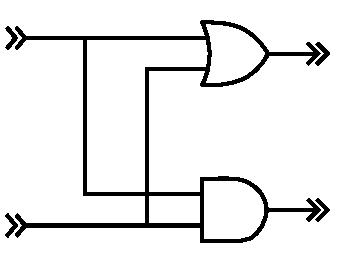
\includegraphics[width= 0.25 \textwidth]{Graphics/1bitCompare.pdf}
\caption{1-bit hardware \texttt{Compare-Exchange}}
\label{fig:bitcompare}
\end{figure}

Sometimes it might be necessary to employ a reverse \texttt{Compare-Exchange} operation, which will swap the elements such that they are in reverse sorted order. Such an operation is obviously just as viable and data-independent as the regular \texttt{Compare-Exchange} operation, but may sometimes give a larger degree of freedom in the description of algorithms.

\subsubsection{Deterministic Data-oblivious Sorting Algorithms}

Deterministic data-oblivious sorting algorithms form a large group of algorithms, though many of them are not known by their data-oblivious qualities, but instead as sorting networks.

\begin{figure}
\center
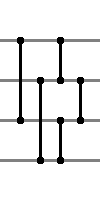
\includegraphics[width= 0.15 \textwidth]{Graphics/network.png}
\caption{4-wire sorting network, equivalent to \texttt{Compare-Exchange} for inputs $(0,2), (1,3), (0,1), (2,3), (1,2)$}
\label{fig:network}
\end{figure}

It is important to note that any fixed sorting network is a data-oblivious sorting algorithm, and can be modelled using \texttt{Compare-Exchange} operations, by performing such an operation for each comparison on the wires of the networks, as seen in Figure\ref{fig:network}. Additionally, any deterministic sorting algorithm depending entirely on \texttt{Compare-Exchange} operations can be viewed as a sorting network that runs a wire for each element of the input, and perform a comparison between wire contents wherever the algorithm performs a \texttt{Compare-Exchange} operation.

Due to their roots in sorting networks, data-oblivious sorting algorithms have a long history, and many algorithms have been developed to perform as sorting networks.

The historical algorithms of Bubble Sort~\citeB{BubbleSort} and the original Shellsort~\citeA{Shellsort} are both examples of simple algorithms that can easily be made data-oblivious by removing any checks for sortedness. This leaves them at their $\Theta(n^2)$ worst-case running time, but makes them easily understandable as data-oblivious algorithms.

Optimal sorting networks have been constructed, running in $\Theta(n \log n)$ time. The most famous of these networks is the AKS sorting network of~\citeA{AKS}, which is widely known, and form the basis of a great deal of research in the sorting networks field. Worth mentioning is also Zig-Zag Sort~\citeA{ZigZag} which is especially interesting due to its simplicity.
These optimal sorting networks are all entirely dependent on the usage of \textepsilon -halvers; a construction that is complicated to produce deterministically, and  has a very high constant factor to their number of comparison. The problem of constructing \textepsilon -halvers makes these optimal sorting networks of little use in practical implementations.

Pratt presents a more efficient variant of Shellsort in his thesis~\citeA{PrattThesis}, that is not only $\Theta(n \log^2 n)$ in the amount of comparisons, but also easily translates into a sorting network. The main idea of Pratt's variant Shellsort, is using a special $\Theta(\log^2 n)$-length jump sequence, instead of the old-fashioned geometric sequences that are often used in Shellsort.

A final interesting family of sorting networks are the algorithms stemming from Batcher's paper on sorting networks~\citeA{SNApplications}, known as Bitonic Sort and Odd-Even Mergesort, along with the Pairwise Sorting Network~\citeA{PairwiseSorting}. These sorting networks achieve sorting at $\Theta(n \log^2 n)$ comparisons, while maintaining a $\Theta(\log^2 n)$ depth, and are simple enough to be implemented on standard hardware, though their asymptotical complexity makes them somewhat lacking when compared to non-oblivious sorting algorithms.

\subsubsection{Randomized Data-Oblivious Sorting Algorithms}

Randomized data-oblivious sorting algorithms are a fairly new development, primarily introduced by \citeA{RandShellSort} and \citeA{AnnealingSort}, but an interesting one. Unfortunately, the list of algorithms performing data-oblivious sorting using a randomized sequence of \texttt{Compare-Exchange} is somewhat short. They are however useful due to the fact that they are simple in their method of operations.

From~\citeA{AnnealingSort} we get Spin-the-bottle Sort and Annealing Sort. The former of which is a $\Theta(n^2 \log n)$ data-oblivious sorting algorithm, of interest only in setting the stage for Annealing Sort, which will with very high probability, sort any given input obliviously in $\Theta(n \log n)$ time.
It is worth noting that the amount of comparisons performed by Annealing Sort has a high constant coefficient if the values given in~\citeA{AnnealingSort} are used, but this could easily be the result of overly pessimistic analysis, as is also the case of~\citeA{RandShellSort}.

A variant of Shellsort, called Shaker Sort is presented in~\citeA{ShakerSort}, and can be implemented as a $\Theta(n \log n)$ sorting network.
Shaker Sort's main deviance from Shellsort is replacing the subsequence sorting with so-called \emph{h-shakes}, which are linear-complexity applications of \texttt{Compare-Exchange} operations up and down the subsequence. Despite having certain bad input permutations, Shaker Sort shows great potential in sorting randomized input data.
By shuffling the input sequence to break up inputs that have been carefully constructed as adversary inputs, we can obtain a randomized variant of Shaker Sort, that  will show excellent performance characteristics, though this requires data-oblivious constructs beyond the \texttt{Compare-Exchange} operation, and will make the algorithm unsuitable for construction as a pure sorting network.

Finally, from~\citeA{RandShellSort} we get Randomized Shellsort, an algorithm that will sort with very high probability in $\Theta(n \log n)$ time by performing \texttt{Compare-Exchange} among random matching pairings taken from regions of the input in regions of sizes matching the subsequence jumps of the original Shellsort algorithm.

Sorting networks can be constructed from randomized data-oblivious algorithms by recording the sequence of operations the algorithm would perform, and constructing the corresponding network. This will lead to networks that use the same amount of comparator components as the amount of \texttt{Compare-Exchange} operations used in algorithm, but the network might not adapt well in terms of depth.

\subsubsection{Algorithms Tabular}

Since the previous subsection includes a great amount of different algorithms, we here present them in short tabular form, as a quick reference sheet.
The table in question is Table~\ref{BigAlgTable}.
\begin{table}[!h]
\begin{adjustwidth}{-.5in}{-.5in}
\centering
\begin{tabular}{|c c c c|}
\hline
Name & Source & Running Time & Keywords \\\hline
Bubble Sort & ~\citeB{BubbleSort} & $\Theta(n^2)$ & Simple \\
Shellsort & ~\citeA{Shellsort} & varies & Customizable, Well-researched \\
AKS Sorting Network & ~\citeA{AKS} & $\Theta(n \log n)$ & Optimal, Theoretical, Depth-optimal \\
Zig-Zag Sort & ~\citeA{ZigZag} & $\Theta(n \log n)$ & Optimal \\
Pratt's Shellsort & ~\citeA{PrattThesis} & $\Theta(n \log^2 n)$ & Shellsort-based\\
Bitonic Sort & ~\citeA{SNApplications} & $\Theta(n \log^2 n)$ & Well-known, Practical \\
Odd-Even Mergesort & ~\citeA{SNApplications} & $\Theta(n \log^2 n)$ & Merge Sort \\
Pairwise Sorting Network & ~\citeA{PairwiseSorting} &  \textcolor{red}{$\Theta(n \log^2 n)$} & Simple \\
Spin-the-bottle Sort & ~\citeA{AnnealingSort} & $\Theta(n^2 \log n)$ & Randomized, Unused \\
Annealing Sort & ~\citeA{AnnealingSort} & $\Theta(n \log n)$ & Randomized, Impractical \\
Shaker Sort & ~\citeA{ShakerSort} & $\Theta(n \log n)$ & Shellsort-Based, Possible~Randomization \\
Randomized Shellsort & ~\citeA{RandShellSort} & $\Theta(n \log n)$ & Randomized, Shellsort-based \\\hline
\end{tabular}
\end{adjustwidth}
\caption{Table of algorithms}
\label{BigAlgTable}
\end{table}